% A template for MCM contest solution
% Make sure 'reedmcm.cls' and 'mcm.sty' are in the directory that you're running latex from.
% These are meant to be used with pdflatex.
% Note: natbib for bibliography.
\documentclass[12pt,draft]{reedmcm}
\usepackage{mcm}
\graphicspath{{./images/}}

%Title
\title{\textbf{The Best Brownie Ever: Finite Difference, Chaotic Maps, and Genetic Algorithms}}
\team{22555} % Put your team control number here. No actual names!
\contest{MCM}
\question{A} % Problem A or B?
\date{\today}

%Headers
\usepackage{fancyhdr}
\pagestyle{myheadings}
\setlength{\headheight}{13.6pt}
\setlength{\headsep}{20pt}
\pagestyle{fancy}
%%% Redefine the plain pagestyle so that it includes the ``page x of
%%% y'' information, as well.
\fancypagestyle{plain}{%
  \fancyhf{} % clear all header and footer fields
  \fancyhead[LO,RE]{Team \# 22555}
  \fancyhead[RO,LE]{Page~\thepage\ of \pageref{LastPage}}
  \fancyfoot[c]{\thepage}
  \renewcommand{\headrulewidth}{0pt}
  \renewcommand{\footrulewidth}{0pt}
}
%%% Define the header as per the contest regulations.
\fancyhead{}
\fancyhead[LO,RE]{Team \# 22555}
\fancyhead[RO,LE]{Page~\thepage\ of \pageref{LastPage}}
\begin{document}

% The Summary of your solution must be on the first page.
%  The contest rules specify that you should include a one-page summary of your report. 
%  You want a brief restatement of the problem followed by a largely \emph{non-technical} description of what you've done.
%  Try to avoid using mathematical notation.
%  You probably want to write a few paragraphs, around half to two-thirds of a page.
%  From COMAP: 
%  "The summary is a very important part of your MCM paper. The
%    judges place considerable weight on the summary, and winning
%    papers are sometimes distinguished from other papers based on
%    the quality of the summary. To write a good summary, imagine
%    that a reader may choose whether to read the body of the paper
%    based on your summary. Thus, a summary should clearly describe
%    your approach to the problem and, most prominently, what your
%    most important conclusions were. The summary should inspire a
%    reader to learn the details of your work.  Your concise
%    presentation of the summary should inspire a reader to learn
%    the details of your work. Summaries that are mere restatements
%    of the contest problem, or are a cut-and-paste boilerplate
%    from the Introduction are generally considered to be
%    weak."

\begin{summary}
  % Aim for three paragraphs
  % 1st: background and GA
  We explore the optimal shape of a baking pan by a genetic algorithm (GA).
  A common shape for a baking pan is rectangle; however, the shape is inferior in terms of temperature distribution, because the heat tends to build up around the corners.
  Circular pans, which do not have this drawback, on the other hand, are less efficient in terms of spatial considerations.
  Thus, our goal is to find a shape that has the best of two worlds: heat distribution and spatial efficiency.
  GA is well-suited for the problem, since our solution space consists of an enormous number of possible shapes.
  Two chaotic area-preserving maps, Arnold's Cat map and Chirikov Standard map, play a crucial role in our GA.
  We use the chaotic transformations to produce various shapes in an almost random manner, a process analogous to generating pseudo-random numbers.
  Furthermore, since the particular chaotic transformations are area-preserving, shapes generated by this process, no matter how different they may appear, have the same area.
  Thus, our GA and the chaotic transformations constitute an effective method for sampling many different shapes, including ones that cannot easily be generated in straightforward methods.
  Our method has the possibility to find an entirely new shape that outperforms conventional shapes in both heat distribution and spatial efficiency.

  % the heat equation model
  The heat distribution on the pan and brownie is computed using the diffusion equation.
  We solve the diffusion equation numerically in SciPy using the finite difference method.
  An analytic solution to the rectangular problem is also explored.
  Parameters of the model were calibrated to reproduce the build-up of heat at the corners of a pan.

  % results and conclusions. . . Definitely write down some numbers
  Varying thermal conductivity of the pan between 1.05 and 200 showed.
\end{summary}
  % End of Summary

% After the Summary, the actual solution starts.
\maketitle
\tableofcontents
\listoffigures
% \listoftables  

\section{Abstract} % Isn't this section redundant since we already have the summary sheet? Can we move it to the end of the intro?
We attempt to implement a model that employs Arnold's cat map to chaotically generate batches of equal-area boundaries in $\mathbb{Z}^2$, which are linearly extended into three dimensional `pans'.  Pans are evaluated using the finite difference method, then culled and recombined by a genetic algorithm in the hope of producing an optimal population.  An analytic solution to the rectangular problem is also explored.

\section{Introduction}
This paper is concerned with modeling and optimization of brownie baking in a standard rectangular oven.
Pans that are commonly used for baking are rectangular; however, rectangle is not an ideal shape when considering the distribution of heat.
Heat tends to build up around the four corner, and the brownie would not be cooked evenly.
To resolve this issue, one may use a circular pan instead.
This shape, however, has limitations, as well.
Since ovens are usually rectangular, circular pans cannot fill the space efficiently, and the amount of goods that can be baked at the same time is reduced by approximately 75\%.
Our goal is to find a pan shape that excel in both heat distribution and spatial efficiency.
Specifically, our model attempts to:
\begin{itemize}
  \item Determine the optimal base shape with regard to the distribution of heat.
  \item Determine the optimal wall shape with regard to the distribution of heat.
  \item Determine the optimal thermal conductivity of the pan with regard to the distribution of heat.
  \item Determine the optimal base shape with regard to the number of pans that can fit in the oven.
\end{itemize}
We attempt to implement a model that employs chaotic transformations to generate batches of equal-area base shapes in $\mathbb{Z}^2$, which are linearly extended into three dimensional `pans'.
Pans are evaluated using numerical solutions of the heat equatiion by the finite difference method, then culled and recombined by a genetic algorithm in the hope of producing an optimal population. 
An analytic solution to the rectangular problem is also explored.

The paper is structures as follows.
First, we discuss the overall picture of our method in the next subsection.
Next, we present assumptions and their justifications, variables, and constants that are incorporated in our model.
Then, we provide backgrounds of the methods used to implement the model.
Finally, we analyze the model and the data obtained from it.

\section{Our Approach: Genetic Algorithm}
Our model employs the following three methods:
\begin{enumerate}
  \item Genetic Algorithm (GA)
  \item Numerically Solving the Dissipation Equation using the Finite Difference Method
  \item Generation of Random Shapes by Area-Preserving Chaotic Maps.
\end{enumerate}
In this section, we discuss GA, the core of our approach, in some detail, and the other two briefly.
The other two are discussed more extensively in later sections. 

GA is an optimization heuristic that mimics the process of natural evolution (Fig~\ref{fig:gaflow}).
GA assigns each pan a \textit{fitness} value based on how close its design is to achieving a set of aims enumerated above (Fig~\ref{fig:fitnessflow}).
%
\begin{figure}[t]
  \centering
  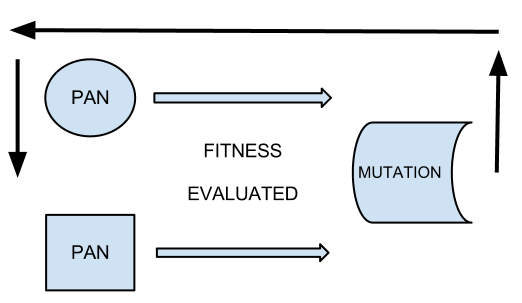
\includegraphics[width=0.5\textwidth]{ga_flowchart}
  \caption{A flow chart of the genetic algorithm.}
  \label{fig:gaflow}
\end{figure}
%
%
\begin{figure}[t]
  \centering
  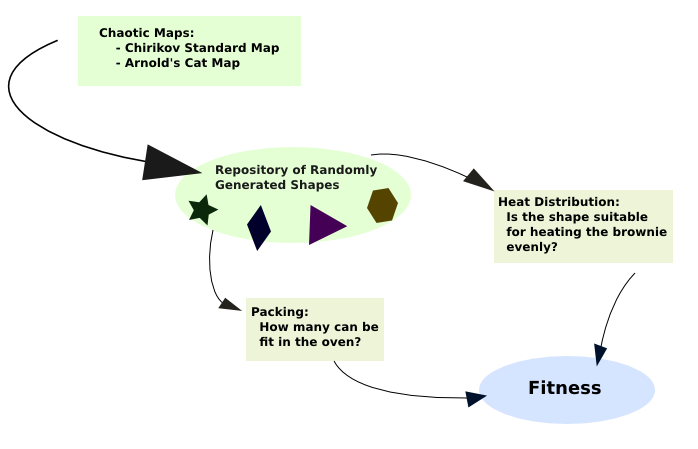
\includegraphics[width=1.0\textwidth]{fitness_flowchart}
  \caption{A flow chart of the generation of shape to the fitness evaluation of a shape.}
  \label{fig:fitnessflow}
\end{figure}
%
The more fit pans are more likely to survive and recombined to form a new pan, which is used in the next iteration of the algorithm. 
After many iterations, we would obtain shapes that satisfy our requirements.
GA is especially suited for searching through a large solution space, which may be computationally infeasible for global optimization algorithms.
This is exactly the case for our problem, since there are practically infinite number of shapes that we can adopt.
Consider the following process that produces a polygon of area $A$:
\begin{enumerate}
  \item Pick a random integer $N \geq 3$.
  \item Pick $N$ points on $\mathbb{R}^2$.
  \item Take the polygon formed by the $N$ points as our shape.
  \item Compute the area of the polygon, and scale it so that the area would become $A$.
\end{enumerate}
This process alone produces an enormous number of different shapes.
Also, it is possible that an optimal pan shape is curvilinear, such as S- or spiral-shaped.
Since GA has the potential to search through a vast solution space, the method allows us to explore shapes that would not be considered in algorithms that require the search space to be reasonably-sized.
Implementations of GA and their benefits as well as limitations are discussed in \citet{mitchell}.

The other major components of our model are area-preserving chaotic maps, and numerical solutions of the diffusion equation.
In short, area-preserving chaotic maps and numerical solutions to the diffusion equation provides our GA means of supplying random shapes and evaluating the fitness of shapes, respectively (Fig~\ref{fig:fitnessflow}).
Later sections discuss the methods in more detail.

\section{The Model}
\subsection{Assumptions and Justifications}
\begin{itemize}
  \item The oven is preheated before the brownies and pan are placed inside, and the temperature of the oven is kept constant by a thermostat. The batter and pan start at equal temperature.

  \item We test a pan one at a time. 
  Even in the case where more than one pans is placed in the oven, our model assumes the sides of our pans are held at constant temperature.  This assumption becomes questionable in a closely packed oven, as the outer pans have more surface area exposed to heat.

  \item The walls of our pans will be flat.
\end{itemize}

\subsection{Variables and Constants}
\begin{itemize}
  \item $n\times m$: grid size
  \item $H$: pan's wall height
  \item $\alpha$: pan's wall slope
  \item $A$: pan's area (Section~\ref{sec:shapes})
  \item $A_{eff}$: the effective area of a shape (Section~\ref{sec:shapes})
  \item $T_{oven}$: the oven's internal temperature
  \item $T_{room}$: the room temperature
  \item $Fit_{total}$: the overall fitness of the shape of a pan (Section~\ref{sec:ga})
  \item $Fit_{pack}$: the fitness of the shape of a pan measured by the number of the same shapes that can be packed in a oven (Section~\ref{sec:ga})
  \item $Fit_{heat}$: the fitness of the shape of a pan measured by reduction in edge overcooking and even heat distribution. (Section~\ref{sec:ga})
  \item $K_{pan}$: the conductivity constant of the pan
  \item $K_{br}$: the conductivity constant of the brownie
\end{itemize}


\section{Genetic Algorithm}
\label{sec:ga}
As we mentioned in the introduction, genetic algorithms (GA) is a crucial piece of our solution.
GA is used to explore an enormous solution space that is made possible by random shape generation by chaotic maps.
Since we have already discussed the overall mechanism of our GA, in this section we define relevant mathematical terms.
These are the three constants that we employ to describe the performance of a shape:
\begin{enumerate}
  \item $Fit_{total}$: the overall fitness of the shape of a pan (Section~\ref{sec:ga})
  \item $Fit_{pack}$: the fitness of the shape of a pan measured by the number of the same shapes that can be packed in a oven (Section~\ref{sec:ga})
  \item $Fit_{heat}$:  the fitness of the shape of a pan measured by reduction in edge overcooking and even heat distribution (Section~\ref{sec:ga})
\end{enumerate}
Our area estimation algorithm (see Section~\ref{sec:shapes}) computes $Fit_{pack}$, and simulation of the heat equation determines $Fit_{heat}$.
$Fit_{total}$ is computed from $Fit_{pack}$ and $Fit_{heat}$ by
\begin{equation*}
  Fit_{total} = w \cdot Fit_{heat} + (1-w) \cdot Fit_{pack},
\end{equation*}
where $w$ is the weight on the requirement of heat distribution, as the problem statement requires.
Thus, when $w$ is large, our GA tends to let shapes with better abilities to distribute heat survive, regardless of their spacial efficiency.

\section{Shapes}
\label{sec:shapes}
The area is fixed to $A$. To determine the optimal shape, we use $A=1$. The effects of varying $A$ are explored separately.

\subsection{Mutation, Area-Preserving Map, and Chaos}
In our GA, mutation serves to introduce new kinds of potential brownie pan base shapes, which are then marked for success or failure by the culinary process of evolution.
We consider mutation as a transformation of a two-dimensional region.
Since pans must be comparable in aptness of packing, we need to mutate shapes in a a way that preserves area.\\
An area-preserving map is a measure-preserving map in a two-dimensional sense, i.e. $m(L^{-1}) = m(L)$, where $m$ is the Lebesgue measure.
For example, suppose $L$ is a linear transformation.
If $\det(L) = 1$ then it is an area-preserving map; the class of such maps correspond to the special linear group $SP(2,R)$.
A typical member of $SP(2,R)$, however, does not bring about a radical change to a shape.
For example, the matrix
\begin{equation*}
\begin{pmatrix}
    \cos\theta & -\sin\theta  \\
    \sin\theta & \cos\theta  
  \end{pmatrix}
\end{equation*}
as a linear map corresponds to the rotation by $\theta$. 
Although this characteristic is suitable as a way of introducing slight modifications to a pre-existing shape, applications of such maps would not create an entirely new shape.
This observation motivates us to employ chaotic maps instead.
We can think of chaotic maps as having a higher mutation rate than non-chaotic maps.
These transformations are deterministic, yet highly unpredictable.
Repeating the application of the chaotic maps a random number of times is, in effect, the very similar to producing random shapes of a fixed area. 
Our process of generating random shapes is similar to a process that generates pseudo-random numbers.
Hence, we can use chaotic maps as a way of creating a random shape, which would correspond to generating a random rational number in a usual GA.
Mutations of shapes by area-preserving chaotic maps allow our GA to explore the solution space that would not be easily accessible otherwise.
In particular, we employ two chaotic maps: the \textbf{cat map} and \textbf{kick map}.

\subsection{The Cat Map}
One of the chaotic maps that we use to mutate shapes is the cat map (commonly refered to as the "Arnold's Cat Map").
Arnold's cat map is a chaotic, area-preserving map on a two-dimensional torus \citep{hilborn}.
The cat map $F$ is defined as
\begin{equation*}
  F: (x,y) \mapsto (2x + y, x + y) \mbox{ (mod 1)}.
\end{equation*}
The corresponding matrix is
\begin{equation*}
A =
\begin{pmatrix}
    2 & 1  \\
    1 & 1  
  \end{pmatrix},
\end{equation*}
and clearly, $\det(A) = 1$.
In order to obtain a wider variety of shapes, we parametrize the Arnold's map as follows:
\begin{equation*}
  F: (x,y) \mapsto (kx + (k-1)y, x + y) \mbox{ (mod 1)},
\end{equation*}
where $k \in \mathbb{R}$, $0 \leq k \leq 10$.
Note that the determinant of the corresponding matrix
\begin{equation*}
\begin{pmatrix}
    k & k-1  \\
    1 & 1  
  \end{pmatrix}
\end{equation*}
is one, and therefore, the parametrized Arnold's map is also area-preserving.
\begin{figure}[p]
  \centering
  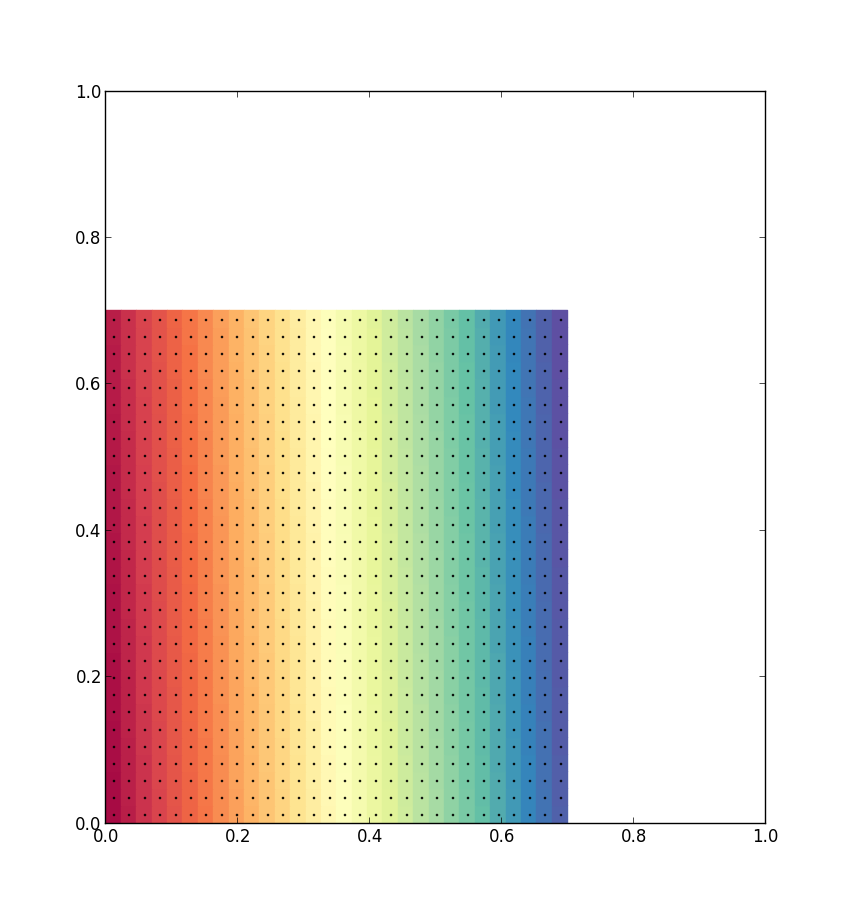
\includegraphics[width=0.5\textwidth]{square_049_900}
  \caption{A square $A = 0.49$ (i.e. the length of each edge is 0.7). Each square consists of patches. This square, for instance, consists of 400 patches, each represented with different colors.}
  \label{fig:square}
\end{figure}
The cat map stretches and folds the domain, and as a result, it produces numbers of thin strips.
The parameter $k$ determines the thickness of the strips;
the higher the value of $k$, the thinner the strips are (Fig.~\ref{fig:catmap_demo1}).
\begin{figure}[p]
  \centering
  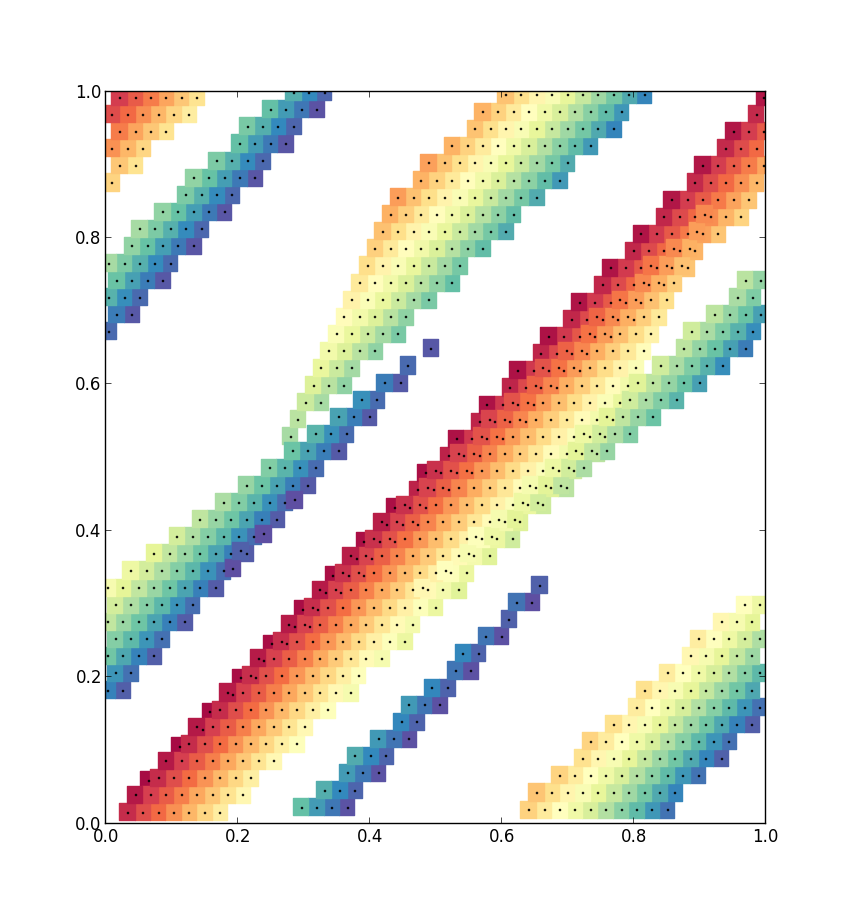
\includegraphics[width=0.4\textwidth]{catmap_1-5}
  \hspace{2cm}
  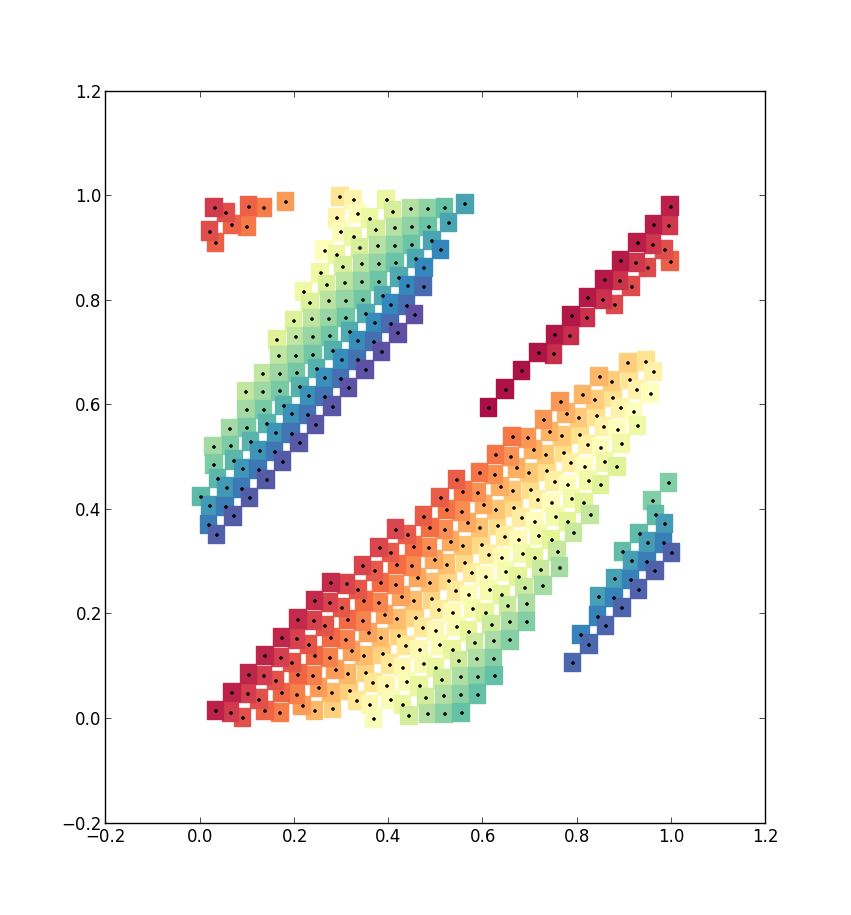
\includegraphics[width=0.4\textwidth]{catmap_3}
  \caption{Cat Map. left: $k=1.5$; right: $k = 3$. After one iteration. 
    Colors of the patches correspond to those in (Fig.~\ref{fig:square}).
    The one with greater $k$ tends to stretch the square to the $x$-direction, and splits the square region into thinner strips.
  }
  \label{fig:catmap_demo1}
\end{figure}
%
Although, $k$ can be any real number, parameters $k_0$ and its negative $-k_0$ result in effectively the same transformation, since the mapped images would be symmetric about the origin, and we take modulus 1 of the points.
Thus, we can only use $k \in \mathbb{R}^+$ without constraining our solution space.
Also, the cat map tends to stretch the unit square to the $x$-direction for greater $k$.
We will use $k \leq 10$, because, in a simulation using a limited precision, $k\geq 10$ does not give rise to appreciably different shapes (Fig.~\ref{fig:catmap_demo2}).

\begin{figure}[h!]
  \centering
  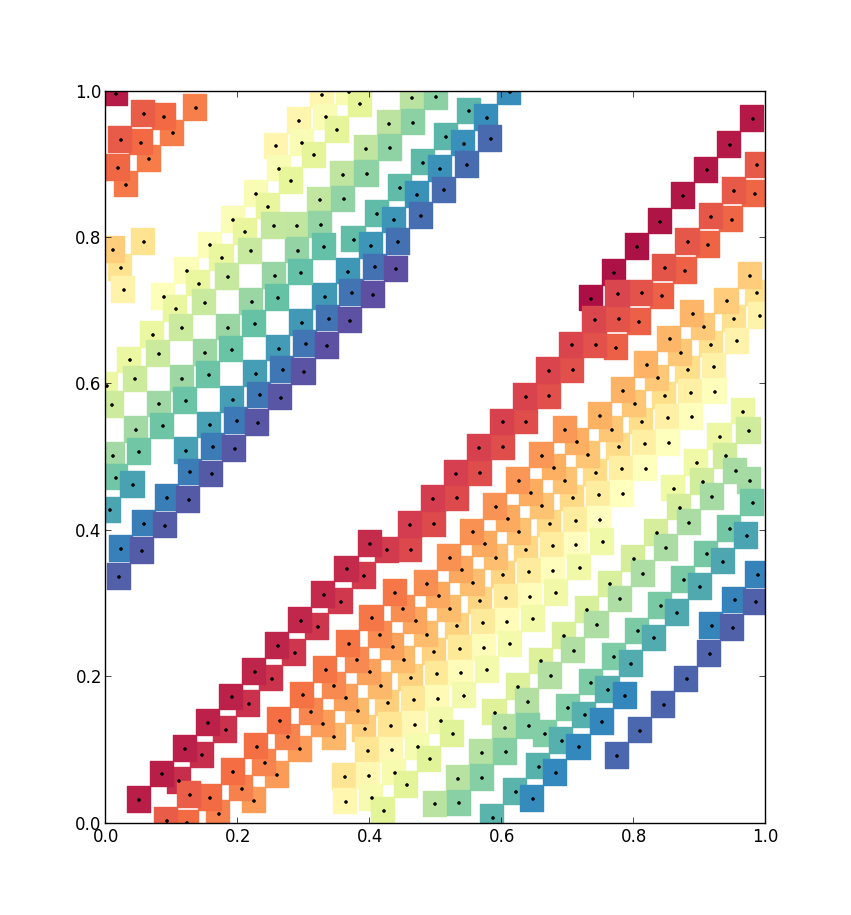
\includegraphics[width=0.4\textwidth]{catmap_10}
  \hspace{2cm}
  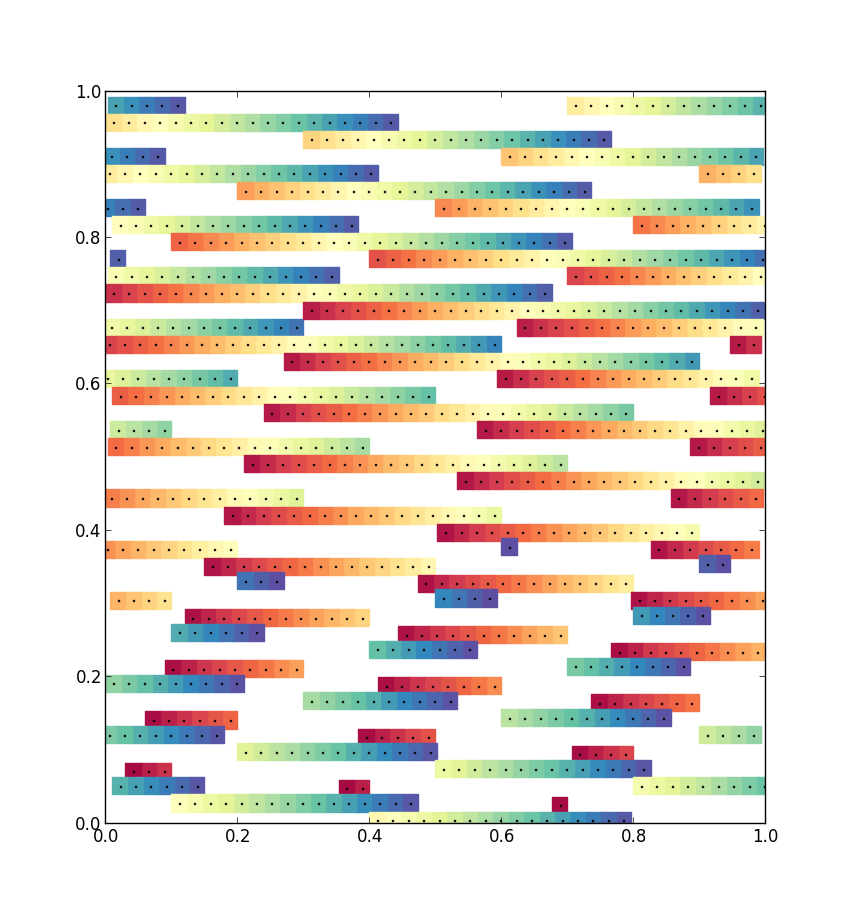
\includegraphics[width=0.4\textwidth]{catmap_30}
  \caption{Cat Map. left: $k=10$; right: $k = 30$. After one iteration. 
    Although the two images are not exactly the same, the differences seem not to be significant from a qualitative point of view.
  }
  \label{fig:catmap_demo2}
\end{figure}

\subsection{The Kick Map}
The other area-preserving chaotic map we employ, the \textit{kick map}, is usually called the Chirikov's Standard Map \citep{ott}.
Qualitatively, the kick map \textit{swirls} a shape, and complements the cat map, whose primary action is \textit{stretching}.
The kick map is defined as:
\begin{align*}
  y &\mapsto y + k \sin x \mbox{ (mod $2\pi$)} \\
  x &\mapsto x + y \mbox{ (mod $2\pi$)},
\end{align*}
where updates of $y$ and $x$ are done asynchronously ($y$ first).
The swirling effects of the kick map are stronger for higher value of $k$ (Fig.~\ref{fig:kickmap_demo1}).
%
\begin{figure}[h!]
  \centering
  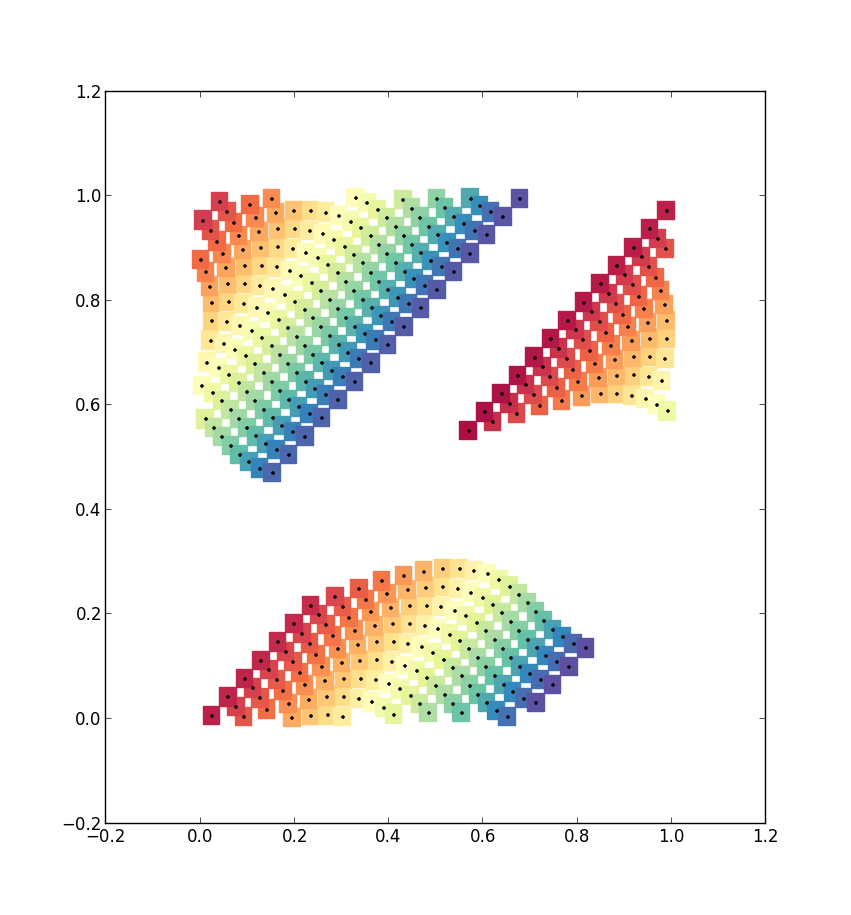
\includegraphics[width=0.4\textwidth]{kickmap_05}
  \hspace{2cm}
  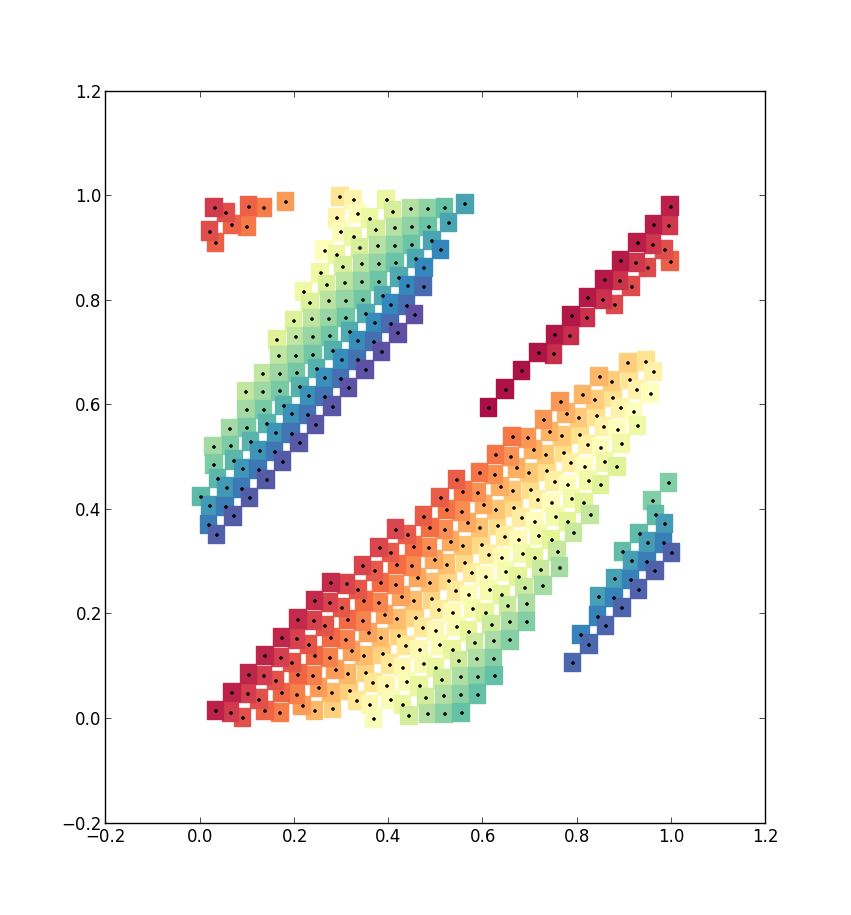
\includegraphics[width=0.4\textwidth]{kickmap_3}
  \caption{The kick map. left: $k=0.5$; right: $k = 3$. After one iteration. 
    The kick map with a higher value of $k$ has stronger effects on the domain.
  }
  \label{fig:kickmap_demo1}
\end{figure}
%
\begin{figure}[h!]
  \centering
  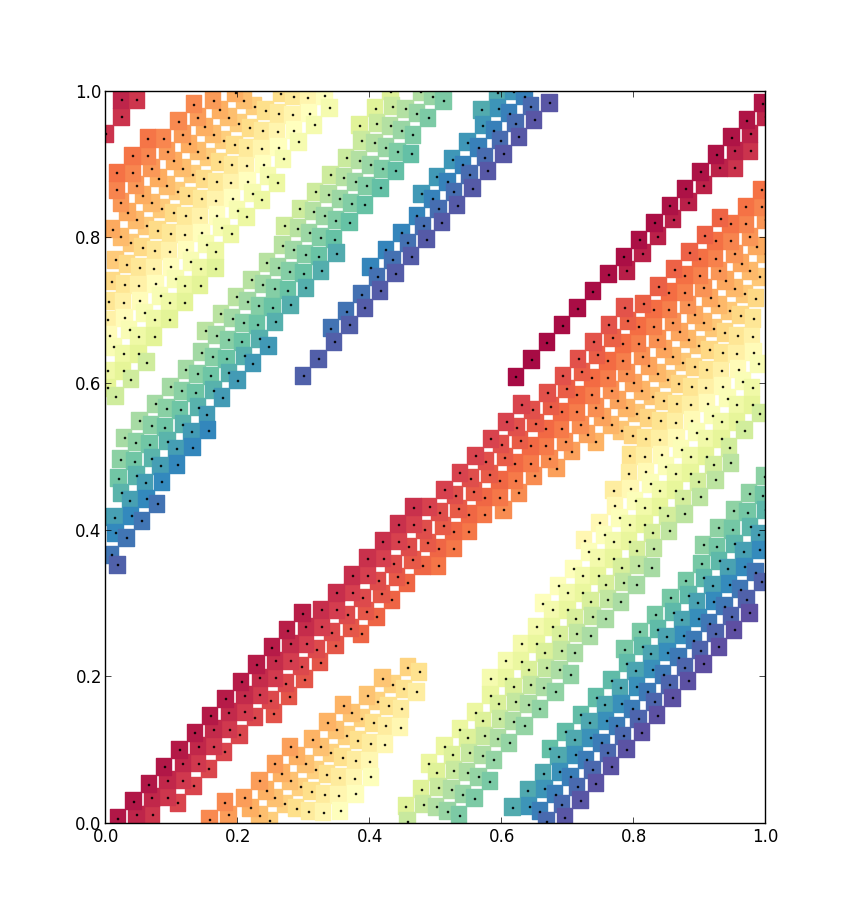
\includegraphics[width=0.4\textwidth]{kickmap_2pi}
  \hspace{2cm}
  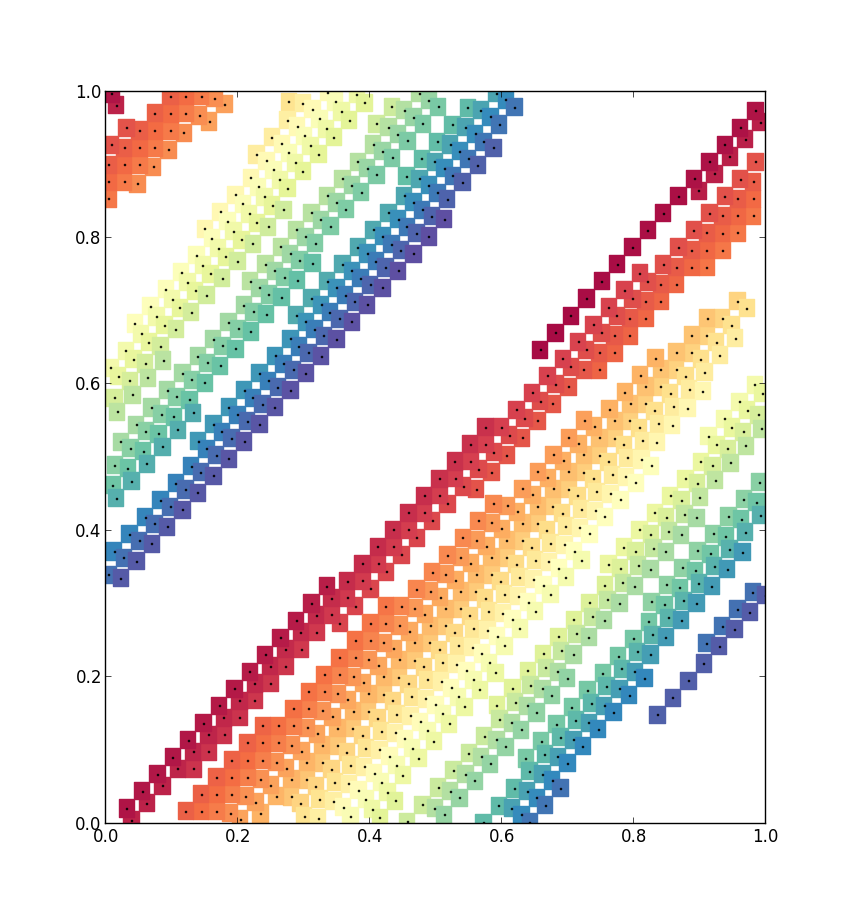
\includegraphics[width=0.4\textwidth]{kickmap_3pi}
  \caption{The kick map. left: $k=10$; right: $k = 30$. After one iteration. 
    Although the two images are not exactly the same, the differences seem not to be significant.
  }
  \label{fig:kickmap_demo2}
\end{figure}
%
As $k$ approaches $1$, the kick map becomes a chaotic chaotic map.
It is known that the chaotic border is $k = 0.971635...$ \citep{spedia}.
Although we would like to apply the kick map to the unit square, the original kick map is a function from $[0,2\pi] \times [0,2\pi]$ to the same region.
We use the following version of the kick map whose domain and image are the unit square:
\begin{align*}
  y &\mapsto \frac{\pi + 2\pi y + k \sin (2\pi x)}{2\pi} \mbox{ (mod 1)}\\
  x &\mapsto \frac{2\pi (x + y)}{2\pi} \mbox{ (mod 1)}.
\end{align*}
In plain words, the coordinates of each point in the unit square are scaled by $2\pi$ prior to the application of the original kick map, then scale the result by $1/2\pi$.
Taking into account of the chaotic border ($k\approx 1$ in the original kick map), we take the range of $k$ to be $(0,2\pi)$.

\subsection{Generation of Random Shapes}
To generate random shapes, we repeatedly apply the chaotic maps to the unit square (Fig.~\ref{fig:square}) $0 \leq k \leq 10$ and $0 \leq k \leq 2\pi$.
In many cases, random iterations result in a chaotic shape that is apparently not suitable as a shape for the pan. 
However, the process may arrive at orderly shapes such as those in Fig.~\ref{fig:order}.
\begin{figure}[h!]
  \centering
  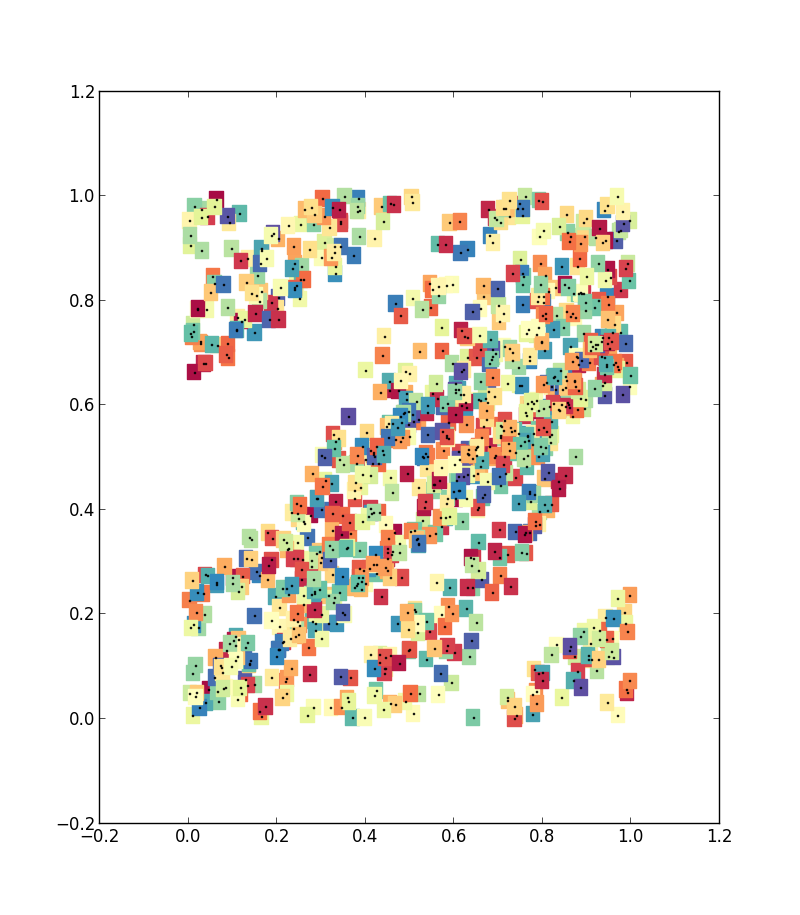
\includegraphics[width=0.4\textwidth]{random2}
  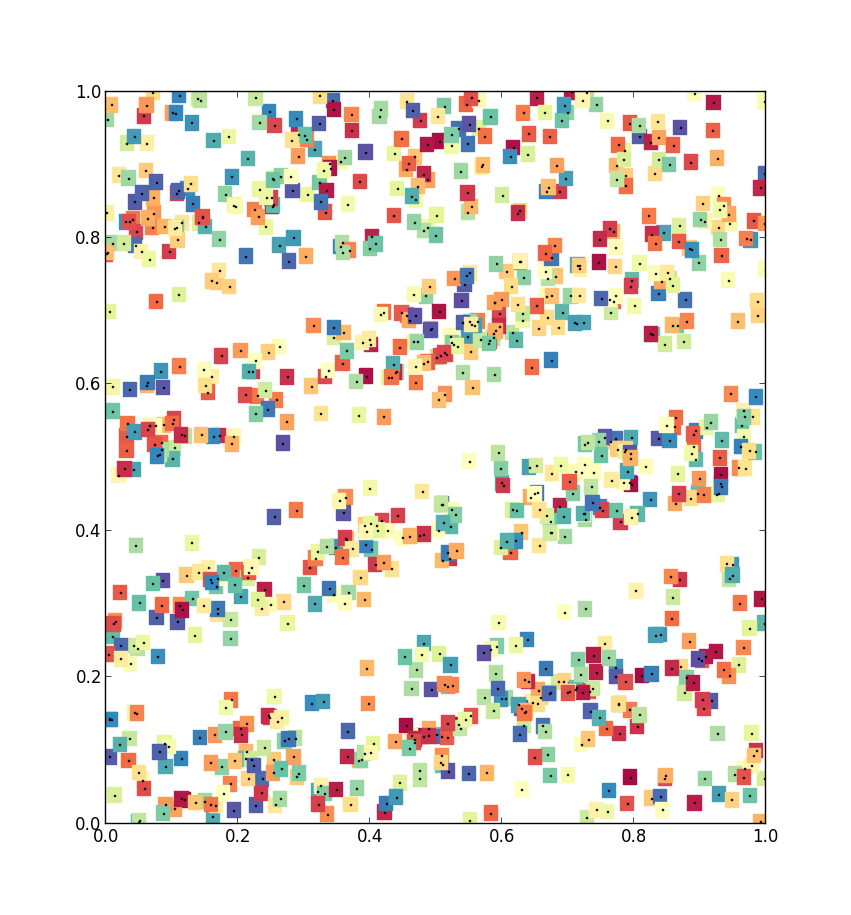
\includegraphics[width=0.4\textwidth]{random128}
  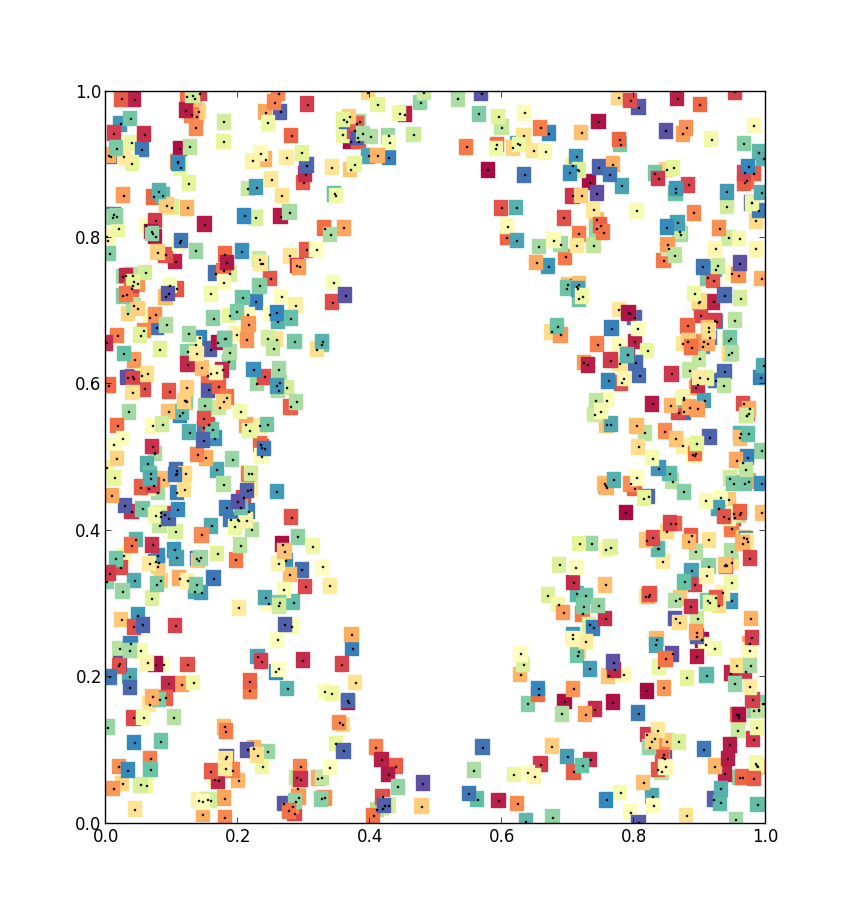
\includegraphics[width=0.4\textwidth]{random256}
  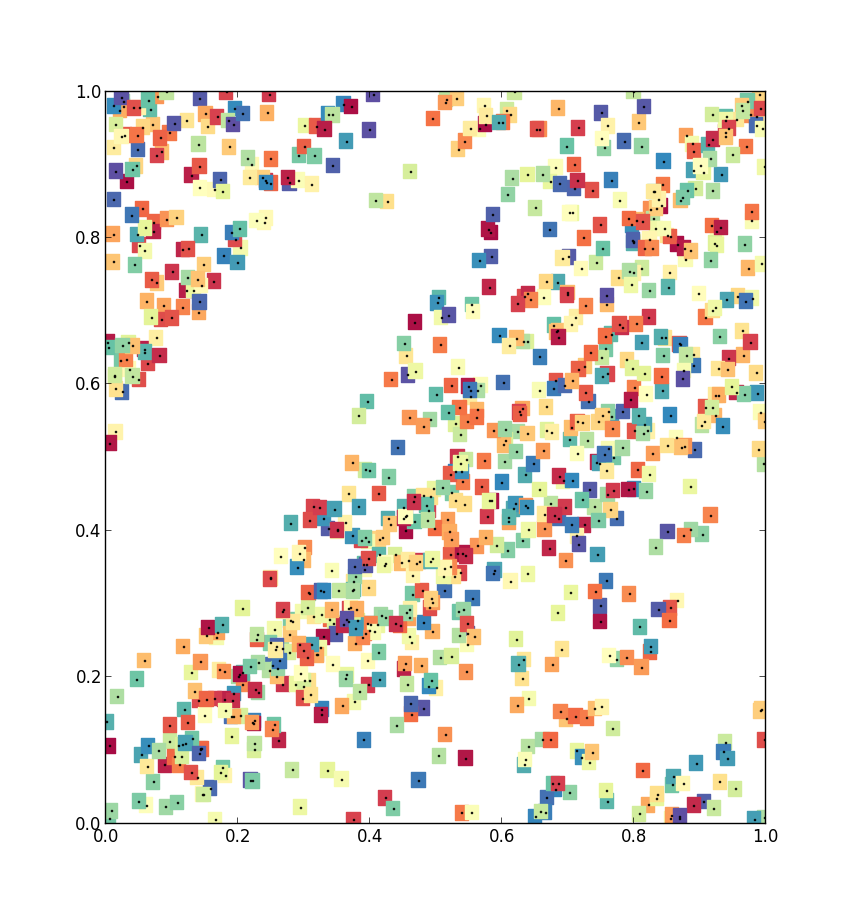
\includegraphics[width=0.4\textwidth]{random1280}
  \caption{Even after random iterations, a process that seem to create a chaos, orderly figures may suddenly emerge.
  These images were produced after random iteration of the chaotic maps 2, 128, 256, and 1280 times, respectively.}
  \label{fig:order}
\end{figure}
%
We see that the repeated random iteration of the cat map and kick map is able to generate random shapes.
We expect that, by this method combined with the genetic algorithm, we may obtain an unforeseen shape that would outperform circular or rectangular pan in terms of both heat distribution and packing efficiency.
\begin{figure}[h!]
  \centering
  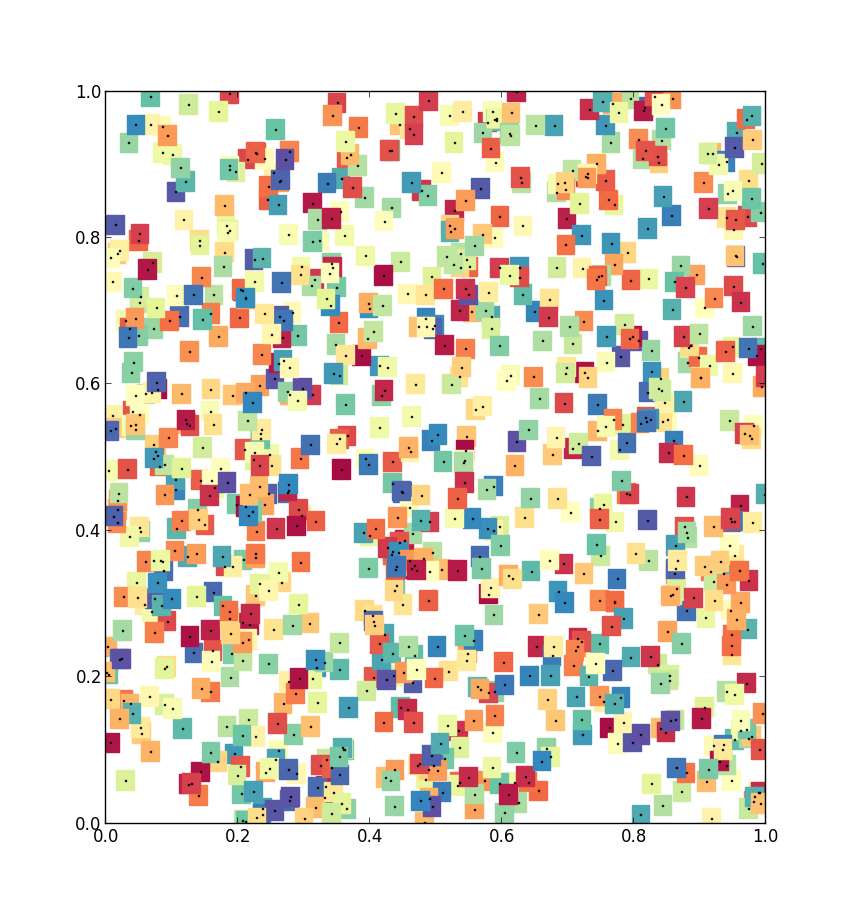
\includegraphics[width=0.5\textwidth]{chaotic_shape}
  \caption{Another example of a square of area 0.64 after 128 random iterations of the cat map and kick map.
  Most of time, random iterations will create a disorderly figure.
  }
  \label{fig:chaotic}
\end{figure}


\subsection{Computing the Boundary}
As we saw in the previous sections, a shape generated by chaotic maps applied to a square is not necessarily a single piece (Fig.~\ref{fig:chaotic}).
We need an algorithm that computes the boundary of a given shape in order to run heat equation simulations for these shapes.
Without knowing the boundary of a shape, we cannot determine the location of walls, which makes simulation impossible.
To compute the boundary of any given shape, we use the \textit{boundary fill algorithm}.
With the knowledge of boundary, we can also check the integrity of a shape in the following manner:
\begin{enumerate}
  \item Pick a point from the collection of patches that constitute a shape.
  \item Perform the boundary fill algorithm to compute the connected components of the point.
  \item Compute the area inside the particular connected component by counting the number of patches in it.
  \item If the area is less than $3A/4$ (the area of the original square), throw away the shape.
  \item Also, if the area is larger than $A$, it means that there are holes on the boundary of the connected component. Such a shape would not function as a pan, so we abandon the shape.
\end{enumerate}
We were not able to include a complete implementation of the boundary fill algorithm in our model.
Because of this limitation, we could not perform the heat equation simulation to determine the heat distribution of a shape, which is a crucial procedure in our GA.
Unfortunately, we were not able to use our genetic algorithm to find an optimal shape.

\section{Packing}
\label{sec:packing}
An ideal shape should fill the oven without creating a waste of space, maximizing the number of pans that can fit in the oven.
Clearly, most of the shapes that our GA generates are not able to form tessellations.
As a measure of how well a shape can pack inside the oven, we use the \textit{effective area}.
The effective area is the area where a shape occupies and cannot be shared with another shape.
For example, if a shape had a hollow circle in the middle, the area would be less than that of the full circle; however, the effective area would be the area of the full circle.
Fig.~\ref{fig:effarea} shows how a shape with empty areas in between can have an effective area larger than $A$.
\begin{figure}[h!]
  \centering
  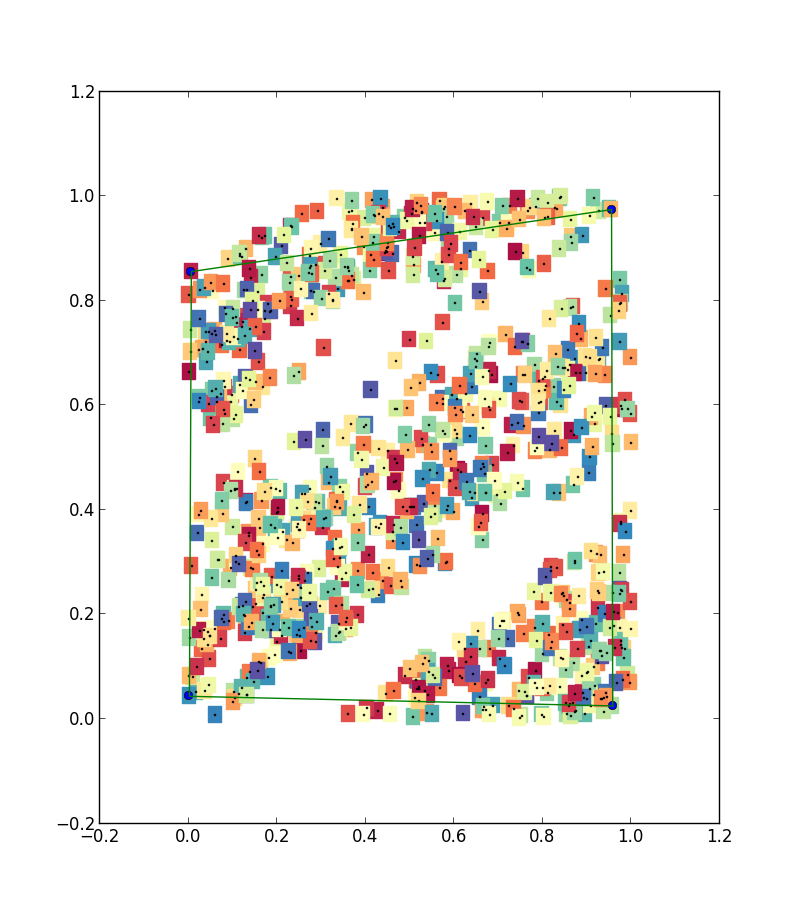
\includegraphics[width=0.5\textwidth]{area_approx}
  \caption{Demonstration of our algorithm to approximate the effective area.
  The area of the square that we started with is 0.81.
  The approximated effective area for this shape is 0.876625844048.}
  \label{fig:effarea}
\end{figure}
%
To approximate the effective area of $A_{eff}$, we do the following:
\begin{enumerate}
  \item Compute the center of mass, which equals to the mean coordinates of all points.
  \item Consider four quadrants around the mean point.
  \item Within each quadrant, compute the point with the greatest distance from the mean point.
  \item The effective area $A_{eff}$ is approximated by a 4-gon with the four vertices.
  \item The fitness $Fit_{pack}$ is $A/A_{eff}$, a rational number less than or equal to $1$.
\end{enumerate}
The area of a quadrilateral defined by the four edges of length $a,b,c,d$ is computed using the \textit{Bretschneider's formula}:
\begin{equation*}
  \frac{1}{4}\sqrt{4p^2 q^2 - (b^2 + d^2 - a^2 - c^2)^2}.
\end{equation*}
The fitness $Fit_{pack}$ is expressed as $A/A_{eff}$.
We have $Fit_{pack} \leq 1$, since $A_{eff}$ is at least as large as $A$.
$Fit_{pack}$ will be used to compute the fitness of a shape together with $Fit_{heat}$.


\section{The Heat Equation}
Our approach began with an attempt to solve the heat equation for a 3D rectangular brownie pan.  Our intent was to first solve the equation for a rectangular mass of brownie batter with unknown boundary conditions on five sides and the upper face held at constant baking temperature $T_b$, and then solve the equation again for the pan around the batter, using the pan solution to fill in the boundary conditions for the batter solution.\\
\\
In hindsight, this approach was misguided for logistical and mathematical reasons.  We spent much time in our first day looking for an exact solution to a specific case that, had we even found it, would not have contributed to our GA-based approach to the general problem.  We also failed to resolve an unknown in the batter solution, which kept us from attempting the second stage of the problem, the pan.  The math issues may have been worsened by our definition of the problem: our boundary conditions held the top of the batter at $T_b$, but the pan and interior brownie batter were given initial temperature $T_i$.  This meant the edges of the batter touching the top of the pan were being held at two inequal temperatures simultaneously, a physical impossibility which at the least seems like a recipe for innaccurate temperature readings around the edges.\\
\\
After we recognized we were spending too much time on it, we gave up on the PDE and switched to the method of finite differences, which proved more successful.  Part 1 of what follows is a discussion of our finite difference solution to the heat problem; Part 2 contains the highlights of a partial solution to the heat equation for the batter mass.\\

\subsection{Numerical Solution}
We implemented the method of finite differences to model the diffusion of heat through the batter and pan using the forward Euler method.  We started in the two-dimensional case, by building a model for a vertical cross section of a rectangular pan, as follows:\\
\\
Let $U^t$ and $C$ be arrays of dimension $M \times N$.  Let $c_a$, $c_p$ and $c_b$ be the thermal conductivity constants of air, the pan material, and brownie batter.  Let $T_i$ stand for the initial temperature of the batter and pan, and let $T_b$ be the baking temperature, which we assume to be constant.  Finally, let $\Delta s = \frac{1}{N}$, and let $w$ be the thickness of the pan material in units.\\
\\
Schematically, we intend $U^t_{i,j}$ to hold the temperature of point $(i,j)$ at time $t$ and $C_{i,j}$ to hold the corresponding thermal conductivity constant.  For an example of initial conditions, consider the $6 \times 6$ case with $w = 1$:
\[U^0 = \begin{pmatrix} T_b&T_b&T_b&T_b&T_b&T_b\\
					T_b&T_i &T_i&T_i&T_i&T_b\\
					T_b&T_i &T_i&T_i&T_i&T_b\\
					T_b&T_i &T_i&T_i&T_i&T_b\\
					T_b&T_i &T_i&T_i&T_i&T_b\\
					T_b&T_b&T_b&T_b&T_b&T_b \end{pmatrix} \hspace{20mm}
  C = \begin{pmatrix} c_a&c_a&c_a&c_a&c_a&c_a\\
				   c_a &c_p &c_b&c_b&c_p&c_a\\
				    c_a &c_p &c_b&c_b&c_p&c_a\\
  				 c_a &c_p &c_b&c_b&c_p&c_a\\
				 c_a &c_p &c_p&c_p&c_p&c_a\\
				c_a&c_a&c_a&c_a&c_a&c_a \end{pmatrix} \]		
To track the evolution of $U$ through time, we define the following partial derivatives for points $(i,j,\tau)$, with time-coordinate $\tau$: \begin{align*}
u_t &\approx \dfrac{u_{i,j}^{\tau+1} - u_{i,j}^\tau}{\Delta t}\\
u_{xx} &\approx \dfrac{u_{i+1,j}^\tau - 2u^\tau{i,j} + u_{i-1,j}^\tau}{(\Delta s)^2}\\
u_{yy} &\approx \dfrac{u_{i,j+1}^\tau - 2u_{i,j}^\tau + u_{i,j-1}^\tau}{(\Delta s)^2} \end{align*}
Given these, the heat equation
\[u_t = c (u_{xx} + u_{yy})\]
becomes
\[\dfrac{u_{i,j}^{\tau+1} - u_{i,j}^\tau}{\Delta t} = c  \left(\dfrac{u_{i+1,j}^\tau - 2u_{i,j}^\tau + u_{i-1,j}^\tau}{(\Delta s)^2} + \dfrac{u_{i,j+1}^\tau - 2u_{i,j}^q\tau + u_{i,j-1}^\tau}{(\Delta s)^2}\right)\]
from which we can derive
\[u_{i,j}^{\tau+1} = u_{i,j}^\tau + c \cdot \frac{\Delta t}{(\Delta s)^2} \left(u_{i+1,j}^\tau + u_{i-1,j}^\tau - 4u_{i,j}^\tau + u_{i,j+1}^\tau + u_{i,j-1}^\tau \right)\]
$\Delta t$, the length of a timestep, can be chosen arbitrarily but must obey the relation
\[\Delta t \leq \frac{(\Delta s)^2}{2c} \text{\citep{horak}}\]
for $c = c_a,c_p,c_b$ for a stable solution.\\


\subsection{Analytic Solution} 
Consider a rectangular mass of batter flush with the first octant and having width $W$, height $H$, and depth $l$.  Let the width of the baking pan be $D$.  Let $K$ be the conduction constant for brownie batter.  Let $T_i$ be the initial temperature of the batter and let $T_b$ be the baking temperature.  Let $f(x,y,z,t)$ be the heat function for the brownie pan, let $r = (x,y,z)$ and let $s = (x + D, y+D, z+D)$ be an `adjustment factor', for later use, so  that the pan problem may also be solved in the first octant.  We wish to find a function $T$ satisfying
\[\partial{T}{t} = K \nabla^2 T\]
subject to the initial condition
\[T(x,y,z,0) = T_i\]
for points in the batter and boundary conditions \begin{align*}
T(0,y,z,t) = T(W,y,z,t) &= f(s,t)\\
T(x,0,z,t) = T(x,L,z,t) &= f(s,t)\\
T(x,y,0,t) &= f(s,t)\\
T(x,y,H,t) &= T_b \end{align*}
where $s$ modifies the coordinates on the term to the left.
To simplify the following computations, we define
\[u(r,t) = T(r,t) - f(s,t)\]
The equation becomes 
\[\frac{\partial u}{\partial t} K \nabla^2 u\]
with initial condition
\[u(r,0) = T_i - f(s,t)\]
and boundary conditions \begin{align*}
T(0,y,z,t) = T(W,y,z,t) &= 0\\
T(x,0,z,t) = T(x,L,z,t) &= 0\\
T(x,y,0,t) &= 0\\
T(x,y,H,t) &= T_b\end{align*}
with the knowledge that $f(x+D, y+D, H+D, t) = 0$, since those points are not part of the pan.\\
\\
Separating variables, suppose
\[u(r,t) = XYZG\]
where $X,Y,Z$, and $G$ are functions of $x,y,z$, and $t$.  We quickly see that \begin{align*}
u_t &= XYZG'\\
u_{xx} &= X''YZG\\
u_{yy} &= XY''ZG\\
u_{zz} &= XYZ''G \end{align*}
Plugging these into the heat equation and dividing by $KXYZG$, we find \begin{align*}
XYZG' &= K(X''YZG +XyY'ZG + XYZ''G)\\
\implies \frac{G'}{KG}  &= \frac{X''}{X} + \frac{Y''}{Y} + \frac{Z''}{Z} \end{align*}
note that the left hand side of this equation is constant, so the right must be as well.  Introducing $\lambda^2$, we write
\[\frac{G'}{KG} = -\lambda^2 \hspace{15mm} \frac{X''}{X} + \frac{Y''}{Y} + \frac{Z''}{Z} = -\lambda^2\]
From the first equation, we immediately get the ODE
\[G'-G\lambda^2 = 0\]
For the others, let
\[\frac{X''}{X} = -\frac{Y''}{Y} - \frac{Z''}{Z} - \lambda^2 = -\mu^2\]
and from there let
\[\frac{Y''}{Y} = -\frac{Z''}{Z} - \lambda^2 + \mu^2 = -\nu^2\]
and
\[\frac{Z''}{Z} = - \lambda^2 + \mu^2 + \nu^2 = -\rho^2\]
\\
We can now derive the following equations: \begin{align*}
X''+ \mu^2 X &= 0\\
Y'' + \nu^2 Y &= 0\\
Z'' + \rho^2 Z &= 0 \\
\mu^2 + \nu^2 + \rho^2 &= \lambda^2
\intertext{and the one from before:}
G'-G\lambda^2 = 0 \end{align*}
The general solution $G$ is $G = A e^{-\lambda^2 K t}$ for some constant $A$.  The general solution for $X'' + \mu^2 X = 0$ is 
\[X = c_1 \cos \mu x + c_2 \sin \mu x\]
Considering the boundary condition $X(0) = 0$, note that $c_1 = 0$.  Considering $X(W) = 0$, we must have $c_2 \sin \mu W = 0$.  Since $c_2=0$ is a trivial case, we focus on cases where $\sin \mu W = 0$.  This happens when $\mu W$ is an integer multiple of $\pi$.  We note therefore that
\[\mu_m = \frac{m \pi}{W}\]
for positive integers $m$.  Substituting these findings into the equation for $X$, we find solutions
\[X_m(x) = \sin(\frac{m \pi x}{W})\]
the same method leads to solutions for $Y$:
\[Y_n(y) = \sin(\frac{n \pi y}{L})\]
for for positive integers $n$.\\
\\
For $Z$, the boundary conditions are $Z(0) = 0$ and $Z(H) = T_b$, so we let
\[Z = \alpha_l e^{\rho_l z} + \beta_l e^{-\rho_l z}\]
the boundary condition $Z(0) = 0$ gives us $\alpha_l = -\beta_l$.  Choosing $\alpha_l = \frac{1}{2}$ we find
\[Z_l(z) = \sinh \rho_l z\]
the separated solution for $u$ is thus
\[u_{mnl}(r,t) = A_{mnl} \sin(\mu_m x) \sin (\nu_n y) \sinh (\rho_l z) e^{-\lambda^2_{mnl}Kt}\]
with
\[\lambda_{mnl}^2 = \mu_m^2 + \nu_n^2 + \rho_l^2 = \left(\frac{m \pi}{W}\right)^2 + \left(\frac{n \pi}{L} \right)^2 + \left(\frac{l \pi}{H}\right)^2\]
We can also form a linear superposition:
\[u(r,t) = \ssum_{m=1}^\infty \ssum_{n=1}^\infty \ssum_{l=1}^\infty A_{mnl} \sin(\mu_m x) \sin (\nu_n y) \sinh (\rho_l z) e^{-\lambda^2_{mnl}Kt}\]
with constants $A_{mnl}$.  This general solution satisfies the boundary conditions on all sides except the top.  To determine the values of the constants $A_{mnl}$, note that at $t = 0$
and therefore
\[T_i - f(s,0) = \ssum_{m,=1}^\infty \ssum_{n=1}^\infty \ssum_{l=1}^\infty A_{mnl} \sin(\mu_m x) \sin (\nu_n y) \sinh (\rho_l z) \]
Let 
\[b_m(y,z) = \ssum_{n=1}^\infty \ssum_{l=1}^\infty A_{mnl} \sin (\nu_n y) \sinh (\rho_l z)\]
and consider the resulting fourier series:
\[T_i - f(s,0) = \ssum_{m=1}^\infty b_m(y,z) \sin (\mu_m x)\]
employing the usual method, we multiply both sides by $\sin (\mu_k x)$ and integrate: \begin{align*}
\int_0^W (T_i - f(s,0)) \sin(\mu_k x) dx &= \ssum_{m=1}^\infty \int_0^W b_m(y,z) \sin(\mu_m x) \sin (\mu_k x) dx
\intertext{Take note that on the right hand side, the sines are orthogonal unless $k = m$, leaving}
\int_0^W (T_i - f(s,0)) \sin(\mu_m x) dx &= \int_0^W b_m(y,z) \sin(\mu_m x) \sin (\mu_k x)\\
&= \frac{b_m(y,z) W}{2}\\
\end{align*}
and so we have 
\[b_m(y,z) = \frac{2}{W} \int_0^W (T_i - f(s,0)) \sin(\mu_m x) dx\]
the same technique will produce the analogous
\[c_n(x,z) = \frac{2}{L} \int_0^L (T_i - f(s,0)) \sin(\mu_n y) dy\]
for the opposite side.\\
\\
We were eventually stumped by the vertical direction.  We searched for a way to use fourier series, defining
\[d_l(x,y) = \ssum_{m=1}^\infty \ssum_{n=1}^\infty \sin(\mu_m x) \sin (\nu n y)\]
so that
\[T_i - f(s,0) = \ssum_{l=1}^\infty d_l(x,y) \sinh (\rho_l z)\]
but couldn't use orthogonality relations on the $\sinh$. We ultimately decided to move on to other methods in the interest of time.\\



\section{Testing and Results}
\subsection{Parameter Fitting}
Using values $m = 10, n=10, T_b = 176, T_i = 15, \Delta t = 1/50000, c_a = .024$, and $c_b = .58$, we varied the conduction coefficient for the pan to attempt to determine the best pan material for even heating around the edges.  Our reasoning in these choices was that $176^\circ C \approx 350^\circ F$ and $15^\circ C \approx 60^\circ F$, representing reasonable estimates for baking temperature and room temperature.  We chose $c_a = .024$ because this is the approximate conduction coefficient of air, although conductivity increases with temperature, so this may be an underestimate in an oven setting.  $c_b = .58$ is approximately the conductivity of water and potatos, which we estimated to be reasonable approximations for brownies.\\

\subsection{Optimal Thermal Conductivity}
We first compared glass ($c_p = 1.05$) to a much less conductive material ($c_p = 0.05$) and aluminum ($c_p = 215$) in a 10x10 grid, and reached the following states in the lower left hand corners after 10000 timesteps (on next page for visual comparison):\newpage
\[c_p = 0.05: \begin{pmatrix} 176&176&176&176&176&176&176&176&176&176\\
176&149.04&152.22&153.46&153.88&154.88&153.46&152.22&149.05&176\\
176&130.22&132.89&133.93&134.26&134.26&133.94&132.90&130.23&176\\
176&119.73&119.45&119.08&118.82&118.82&119.08&119.45&119.73&176\\
176&114.59&111.31&109.25&108.24&108.24&109.25&111.31&114.59&176\\
176&112.76&107.61&104.24&102.57&102.58&104.24&107.61&112.76&176\\
176&113.96&107.97&103.68&101.55&101.55&103.68&107.98&113.97&176\\
176&120.22&112.47&107.11&104.67&104.67&107.12&112.47&120.23&176\\
176&137.07&120.13&113.46&111.28&111.28&113.46&120.13&137.07&176\\
176&176&176&176&176&176&176&176&176&176\end{pmatrix}\]


\[c_p = 1.05: \begin{pmatrix} 176&176&176&176&176&176&176&176&176&176\\
176&174.52&173.06&171.97&171.39&171.39&171.97&173.06&174.52&176\\
176&173.22&170.47&168.43&167.34&167.34&168.43&170.48&173.22&176\\
176&173.22&170.47&168.43&167.34&167.34&168.43&170.48&173.22&176\\
176&172.26&168.57&165.83&164.36&164.36&165.83&168.58&172.26&176\\
176&171.76&167.59&164.48&162.82&162.82&164.48&167.29&171.77&176\\
176&171.76&167.64&164.55&162.90&162.90&164.55&167.59&171.79&176\\
176&172.33&168.72&166.03&164.59&164.60&166.03&168.72&172.33&176\\
176&173.32&170.70&168.74&167.69&167.70&168.74&170.70&173.32&176\\
176&174.61&173.32&172.34&171.82&171.82&172.34&173.32&174.61&176\\
176&176&176&176&176&176&176&176&176&176\end{pmatrix}\]
\[c_p = 215: \begin{pmatrix} 176&176&176&176&176&176&176&176&176&176\\
176&174.84&173.52&172.54&172.01&172.02&172.54&173.53&174.84&176\\
176&173.82&171.36&169.52&168.53&168.53&169.52&171.36&173.82&176\\
176&173.08&168.78&167.31&165.99&166&167.32&169.79&173.08&176\\
176&172.7&168.99&166.21&164.72&164.72&166.21&169&172.71&176\\
176&172.74&169.08&166.33&164.86&164.87&166.34&169.08&172.75&176\\
176&173.19&170.04&167.68&166.41&166.42&167.68&170.04&173.19&176\\
176&173.98&171.74&170.07&169.17&169.17&170.07&171.75&173.98&176\\
176&174.99&173.99&173.21&172.79&172.8&173.21&173.99&174.99&176\\
176&176&176&176&176&176&176&176&176&176 \end{pmatrix}\]
\\
In each of these cases, the open top of the pan is oriented upward.  Observing results of the simulation, we were suprised by the relatively small difference between glass and aluminum, despite the apparently large difference in conductivity.  We took the variances of the batter in the aluminum and glass pans above and found them to be 12.18 and 9.26, respectively.  An $F$-test found this difference to be insignificant, with a p-value of $0.09$.
From this we concluded from this that, assuming a minimal level of conductivity (on par with glass), an increase in conductivity does little to increase or allay heat buildup around the edges of the pan.\\
\\
Our next step was to design an analogous scheme for the three-dimensional problem.  Using the partial derivatives
\begin{align*}
u_t &\approx \dfrac{u_{i,j,k}^{q+1} - u_{i,j,k}^q}{\Delta t}\\
u_{xx} &\approx \dfrac{u_{i+1,j,k}^q - 2u^q{i,j,k} + u_{i-1,j,k}^q}{(\Delta s)^2}\\
u_{yy} &\approx \dfrac{u_{i,j+1,k}^q - 2u_{i,j,k}^q + u_{i,j-1,k}^q}{(\Delta s)^2}\\
u_{zz} &\approx \dfrac{u_{i,j,k+1}^q - 2u_{i,j,k}^q + u_{i,j,k-1}^q}{(\Delta s)^2} \end{align*} 
we arrived at the 'update function'
\[u^{q+1}_{i,j,k} = u^q_{i,j,k} + c \frac{\Delta t}{(\Delta s)^2} \left(u^q_{i+1,j,k} + u^q_{i,j+1,l} + u^q_{i,j,k+1} + u^q_{i-1,j,k} + u^q_{i,j-1,k} + u^q_{i,j,k-1} - 6u^q_{i,j,k} \right)\]
and successfully replicated heat buildup around the edges and corners of the brownie pan.\\
\\



\subsection{Strengths and Weaknesses}

\section{Conclusion}
Our essential plan was to use Arnold's cat map to generate batches of random shape boundaries, then extend the boundaries upward at a linear slope to form three dimensional 'pans' to be evaluated for effectiveness using finite differences.  We would have then used a genetic algorithm to cull the most ineffective pans from the population.  We ran into unexpected difficulty when faced with the problem, given an arbitrary and possibly disjoint boundary, of deciding whether points in the oven lie within the boundary or outside it.  This undermined our ability to differentiate between batter and air in our model oven.  The next step would have been to generalize the finite difference scheme for arbitrary shapes, but due to time and practical constraints we were unable to implement our final plans. 

In order to improve our model
\begin{enumerate}
  \item Need to implement an algorithm to connected-components. Flood-fill algorithm is an example of such an algorithm.
  \item recompute variances with batter NOT including pan! M[2:-2,2:-2]
\end{enumerate}

% The bibliography is in a separate file
\renewcommand{\bibname}{References}
\bibliographystyle{plainnat}
\nocite{*}
\bibliography{mcmbib}

\end{document}
